\section{Data storage and management system}

\subsection{The \pdsp data characteristics}
Characteristics of the \pdsp data are in large part defined by a few fundamental
properties of the \pdsp Liquid Argon TPC:
\begin{itemize}
\item the high spatial granularity of the detector (e.g., the pitch of the wires, etc), and the resulting high channel count;
\item high digitization frequency (which is essential to ensure a precise position measurement along the drift direction); and
\item relatively slow drift velocity of electrons in LAr, which requires a substantial readout window (of the order of milliseconds)  to collect
all of the ionization in the LAr volume stemming from the event of interest and overlapping cosmic rays.
\end{itemize}

%\noindent 
Triggered readouts of the detector, denoted ``events'' here, 
thus contain a significant amount of raw data, impacting the bandwidth and
storage requirements.   The run plan, which determines the total number of required events, 
helps define the design requirements for the data storage and management system.

The \textit{``\pdsp Data Scenarios''} spreadsheet\,\cite{data_spreadsheet}  %(DUNE DocDB 1086)
describes a few possible running conditions. It includes estimates for their
resulting data volumes and rates, and interpretations of these estimates in terms of
network and disk bandwidth. The set of conditions labeled as ``Central'' represents the most likely scenario
and is correlated with the current run plan (see Section~\ref{sec:runplan}).
% maxim: fixed
% \fixme{Should briefly describe what the 3 running conditions are}
 It also includes estimates for non-beam
data in order to constrain the contributions of cosmic rays to the beam-on data.  Some highlights
of these estimates for the ``most likely'' scenario
can be found in Table~\ref{tab:goldi}.

Based on the estimated event-readout size quoted in Table~\ref{tab:goldi}  the anticipated raw data volume to be taken during the planned SPS run
amounts to about 3\,PB.


%%%%%%%%%%%%%%% Tom's stuff
\subsection{Interface of the DAQ to the online storage}
\label{sec:DAQ_online_interface}

%Table\,\ref{tab:goldi} indicates a nominal trigger rate of 25\,Hz for the mid-range scenario. It may be necessary to provide the capability to run at  an instantaneous trigger rate of up to 100\,Hz in order to allow for commissioning and schedule delays. For that reason, scalability of the DAQ, the online buffer and the prompt processing system \ref{sec:prompt_processing} is an important design requirement. Data are assumed to be collected based on prompt trigger signals generated by the beamline instrumentation in order to purify samples of desired particles.
Table\,\ref{tab:goldi} indicates a nominal trigger rate of 25\,Hz for
the mid-range scenario. It may be necessary to provide the capability
to run at  an instantaneous trigger rate of up to 100\,Hz in order to
allow for commissioning and schedule delays. For that reason,
scalability of the DAQ, the online buffer and the prompt processing system
(Section~\ref{sec:prompt_processing}) is an important design requirement.
 Data are assumed to be
collected based on prompt trigger signals generated by the beamline
instrumentation in order to purify samples of desired particles.

%Current estimates put the PDS data at approximately 10\% of the TPC data rate.  Beam instrumentation data is expected to be lower still. As such, the readout of the photon detector channels and the beam instrumentation is assumed to be a relatively minor addition to the total data rate and are not anticipated to drive the design of the data handling and processing system, although adequate resources must be provisioned in order to acquire and store the data from these systems. 
Current estimates put the PDS data at approximately 10\% 
of the TPC data rate.  Beam instrumentation data is expected to be lower still.
Although adding to the
total data rate only slightly, adequate resources must
be provisioned in order to acquire and store the data from these
systems.  

The network speed of all computers in the DAQ
chain is anticipated to be 20\,Gbits/sec. 
 Computers running near-line
processing of subsets of the data, which are generally CPU-bound, may
be connected with 1\,GBit/sec links.  The software framework for
interfacing with the electronics, building events, writing data files,
and providing an interface to online monitoring of data as it is
acquired is {\it artdaq}~\cite{artdaq}.

%Assuming that each RCE reads out 256 channels of the TPC, 60 RCE's will need to be active.  For the PDS, 24 SSPs will be used.  A number of computers (minimum 2) running BoardReader processes will read out the RCEs.  These computers should be provisioned with 1 core per process, along with a 10\,Gbit/sec network connection.  The BoardReader processes will transmit data to a set of computers running EventBuilder processes. A number of Event Builder computers (minimum 4), with 10-20 cores and a pair of 10\,Gbit/sec NIC will provide the CPU and networking needed to build events, collect basic metadata, and send the data to storage and online monitoring.  The Event Builders assemble data fragments sent by the BoardReaders into self-consistent events consisting of readout data from each contributing RCE, SSP, and beam instrumentation information for the same time period.  They will also perform basic data integrity checks, ensuring that all data that are expected for an event have arrived and have not been corrupted, before writing records out.

Given that each RCE reads out 256 channels of the TPC, 60 RCEs
will need to be active.  For the PDS, 24 SSPs will be used.  At least two computers 
running BoardReader processes will read out
the RCEs and transmit data to a set of computers running EventBuilder processes.
These computers and a
pair of 10\,Gbit/sec NIC will provide the CPU and networking needed to
build events, collect basic metadata, and send the data to storage and
online monitoring.  
The Event Builders assemble data fragments into self-consistent events and perform basic data integrity checks before writing records out.

%do not change following pgraph
The online buffer layer will consist of $\sim$300\,TB of storage,
which will be connected directly to the Event Builders.  The baseline
storage option consists of two SAS arrays DAS with $>40$Gbit/s bandwidth,
redundant paths, controllers, and power supplies.
A backup option for storage is an XRootD cluster~\cite{xrootd} taking
data directly from the Event Builders over the network.

After the data are written to disk by {\it artdaq}, the data handling
system creates metadata files,optionally  runs near-line monitoring jobs, and
transfers the data from EHN1 to the CERN Computing Centre \cite{docdb1212}.
The ``Fermi File Transfer Service'' (F-FTS) software 
developed and maintained at FNAL will be the central element
of the data flow management at this level.

%%%%%%%%%%%%%%%%%%%%%%%%
\subsection{Raw data flow in \pdsp}
\label{sec:raw_concept}

\begin{figure}[tbh]
\centering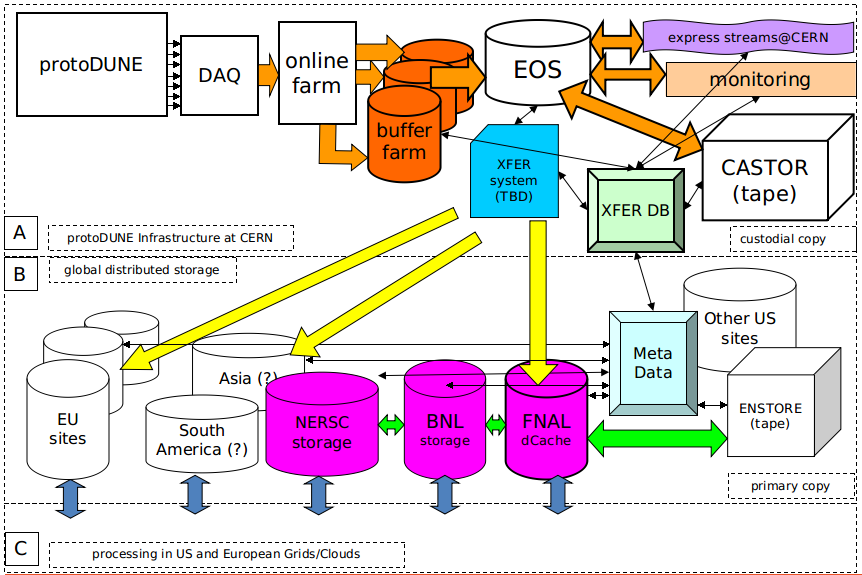
\includegraphics[width=\linewidth]{protoDUNE_raw_data_concept.png}
\caption{\label{fig:raw_concept}Conceptual diagram of the flow of raw data in \pdsp}
\end{figure}


%\noindent
A conceptual diagram of the raw data flow in \pdsp is presented in Figure~\ref{fig:raw_concept}. It shows the general logic
of the data flow and does not rely on assumptions of specific technical implementations. 
It also reflects the central role of CERN EOS in the \pdsp raw data management scheme which is motivated by the experience
and architecture of the LHC experiments.

EOS serves as the staging area from which the data are committed to CASTOR
and from which data are transmitted to a number of endpoints including principal data centers such as FNAL and others.
It is also used to provide input to QA and other express processing streams at CERN (Section~\ref{sec:prompt_processing}).
%This scheme assumes that there is no conceptual difference between NP02 and NP04 in terms of the general pattern of data flow.

Data centers at BNL and National Energy Research Scientific Computing Center (NERSC)
are placed in this diagram for illustration purposes. Any other institution possessing adequate
resources can participate in this data distribution scheme if desired.
\fixme{Thomas: This may trigger the question whether we can harvest such pre-existing resources at other institutions. Do we know what exists and is available ? Do we have a plan or are we ignoring this for now ?}
-
\fixme{Maxim: the answer to harvesting is "maybe". It is a possibility, remains to be seen how to materialize it. It's worth mentioning that we'll be likely resource-hungry.}
 This part of the data transmission process will be handled by an instance of F-FTS~\cite{docdb1212}.



